\chapter{Beschreibung des Endproduktes}\label{cha:theoretical-background}
\pagebreak 
\section{Brillenkategorien}
Über den Menüpunkt "Home" gelangt man zu einer Übersicht aller Brillenkategorien. Dies ist gleichzeitig die Hauptseite der Webseite. Wird eine der 3 Kategorie (Herrenbrillen, Damenbrillen und Kinderbrillen) ausgewählt so werden die dazugehörigen Brillen auf einer neuen Seite angezeigt.

\begin{figure}[H]
\begin{center}
	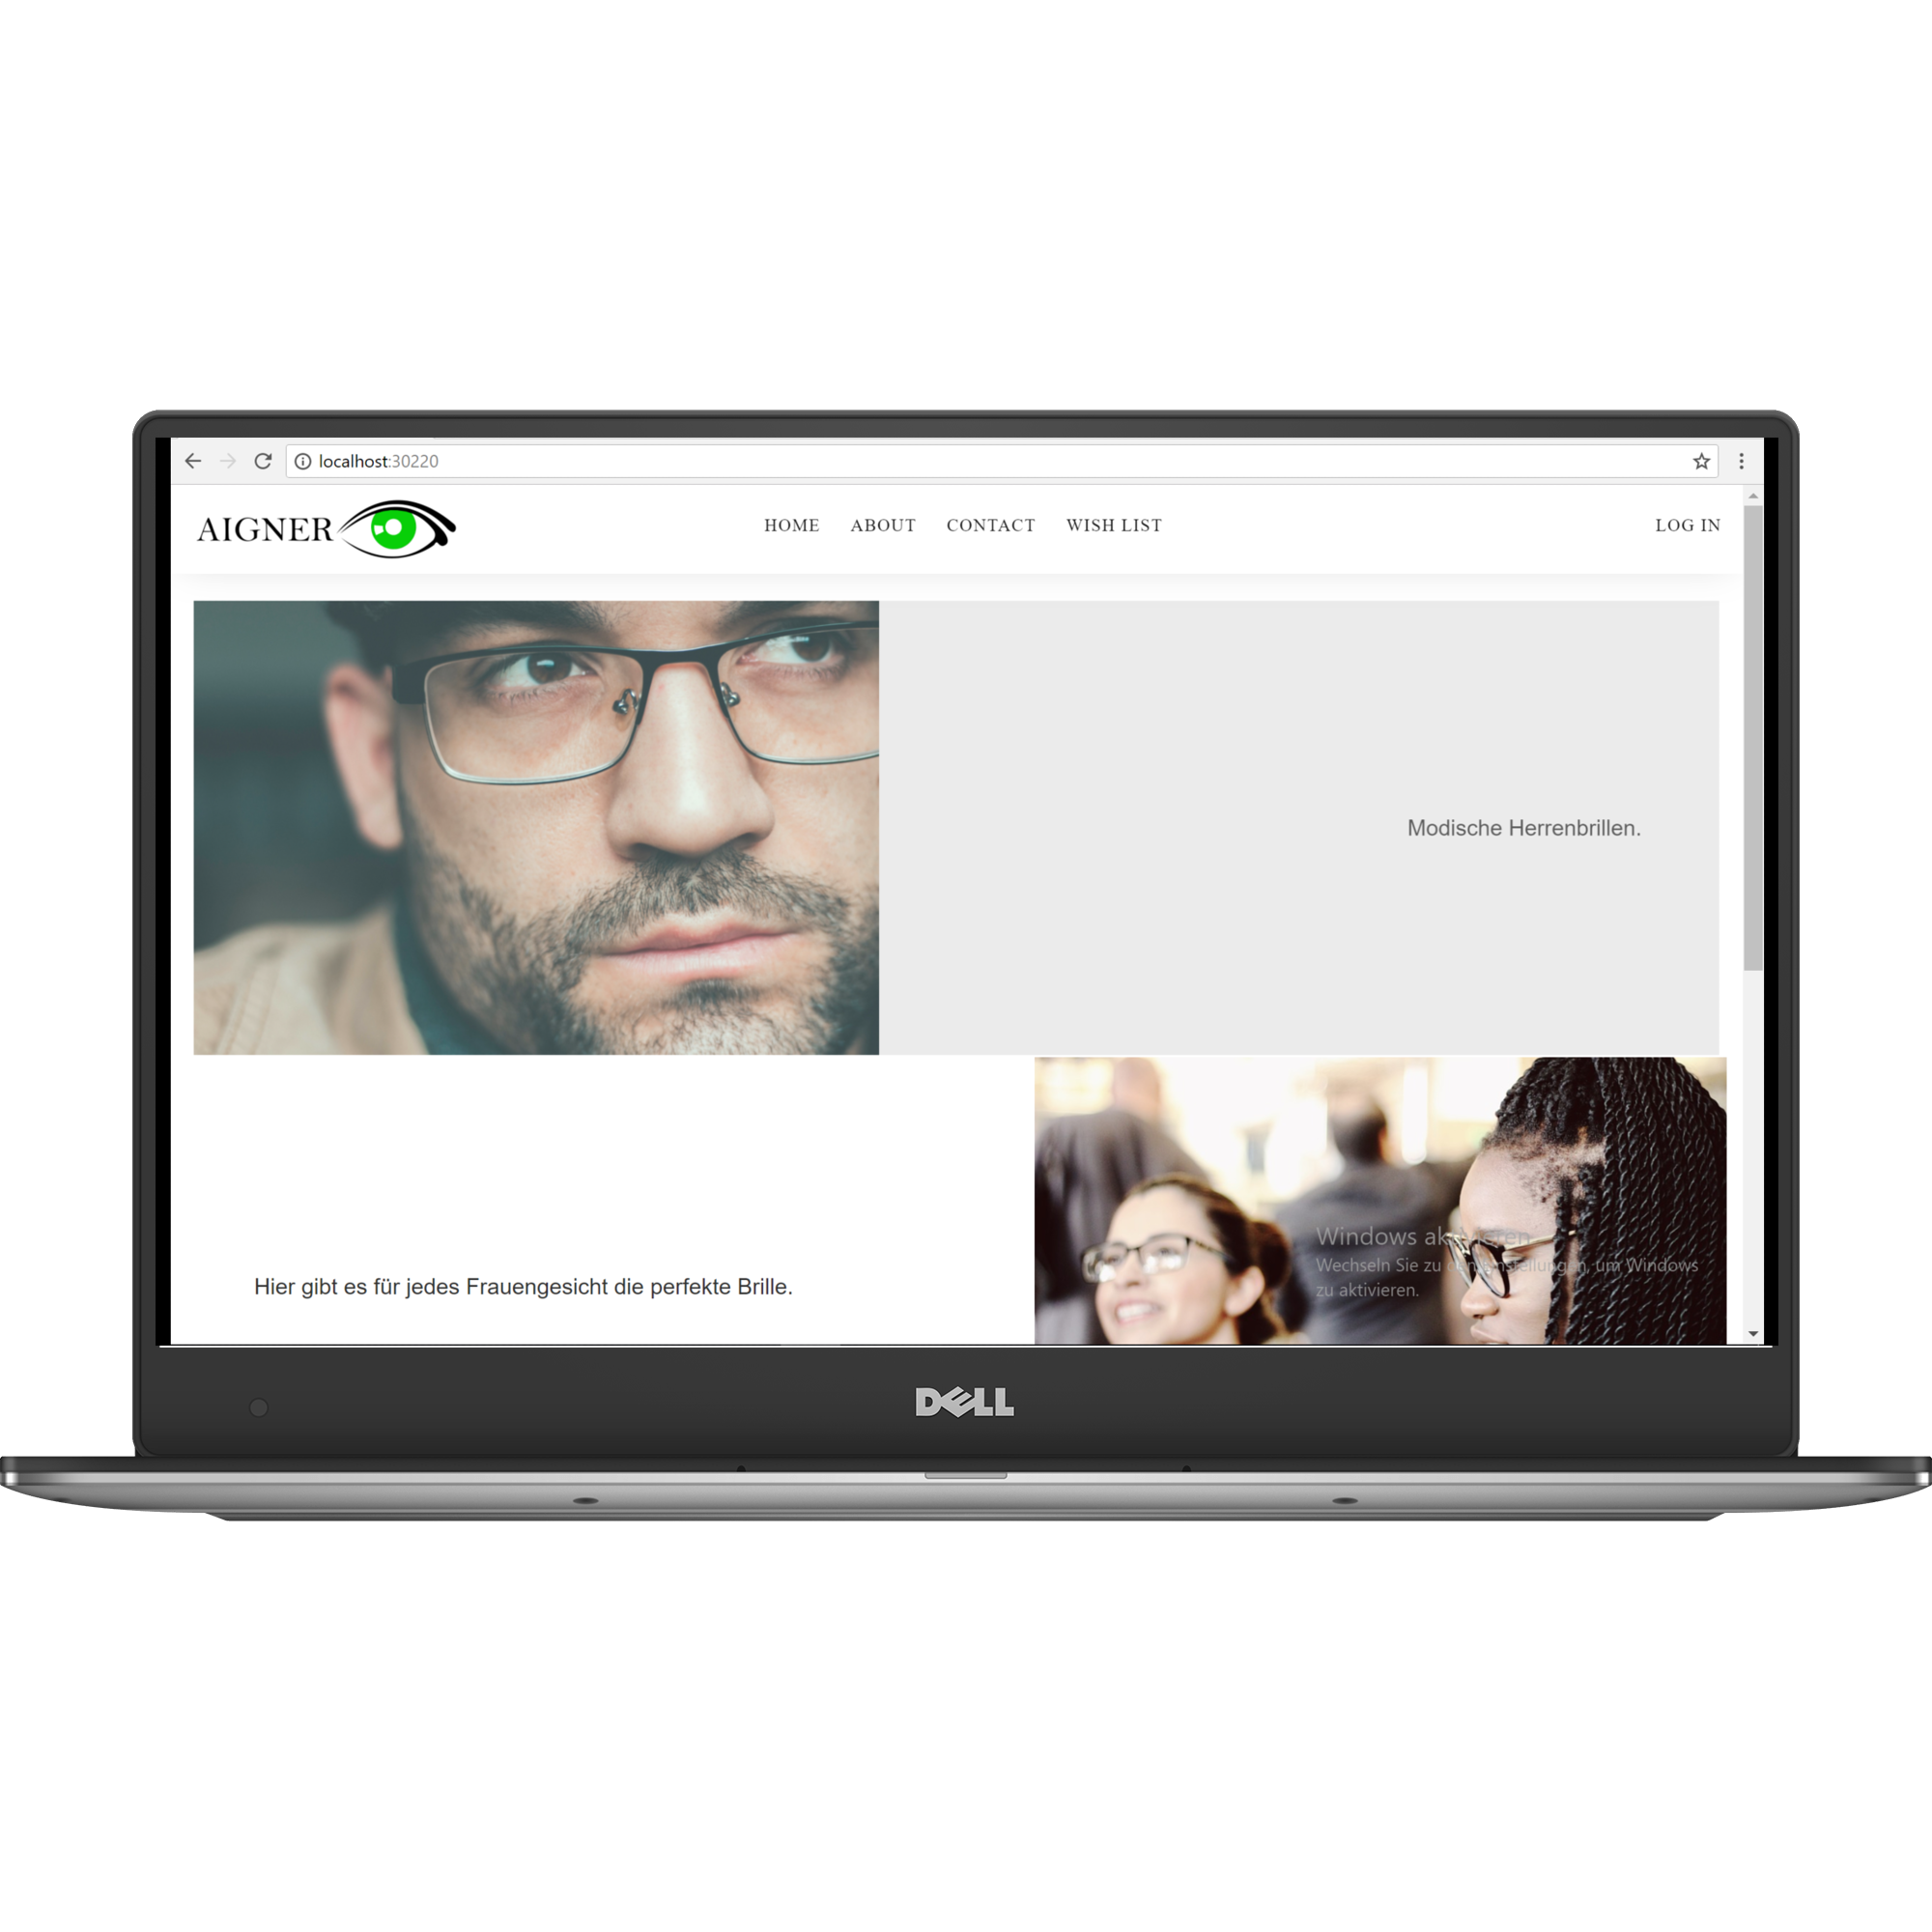
\includegraphics[scale=.2]{images/Index.png}
\end{center}
	\caption{Brillenkategorien}
	\label{fig:sample}
\end{figure}
\pagebreak
\subsection{Brillenmodelle}
Die Brillenmodelle sind in drei Kategorien untergliedert "Herrenbrillen" , "Frauenbrillen" und "Kinderbrillen" auf jeder der Unterseiten werden die dazugehörigen Brillen mit einem Foto, dem Titel und dem Preis dargestellt. Jede Brille kann dann einzeln mittels eines Buttons auf den Wunshzettel gesetzt werden.
Die Brillenmodelle werden nach der Kategorie gefiltert. Auf der "Home" Seite wird eine Kategorie ausgewählt alle Brillenmodelle die diese Kategorie haben werden angezeigt.
Jedes Brillenmodell hat einen Preis nach belieben können die Brillen nach dem Preis auf- oder absteigend sortiert werden. 

\begin{figure}[H]
\begin{center}
	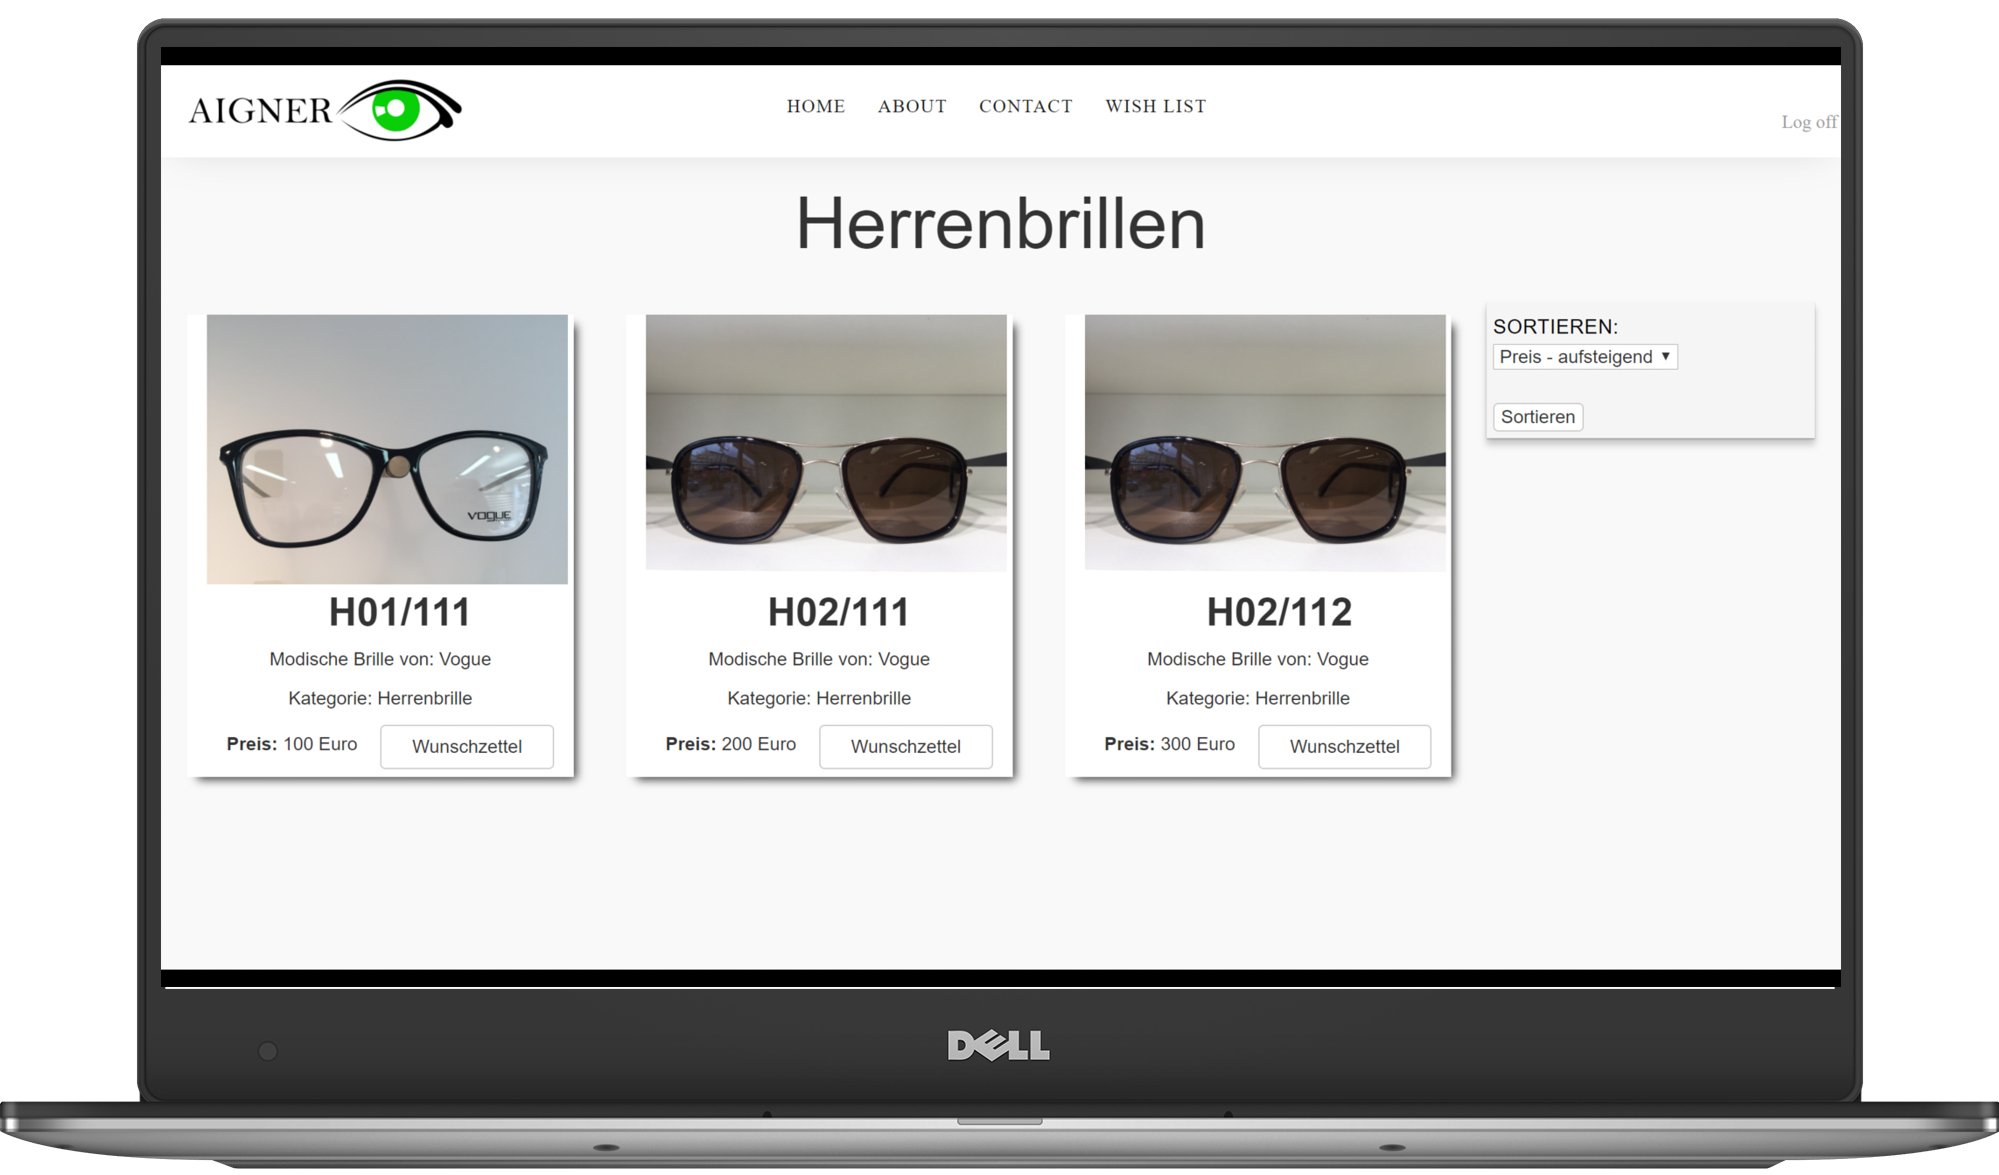
\includegraphics[scale=.2]{images/Brillen.png}
\end{center}
	\caption{Model-View-Controller Konzept}
	\label{fig:sample}
\end{figure}


\section{Wunschzettel}
Unter dem Punkt "Wunschzettel" auf der Navigation bar findet man alle Brillenmodelle die man zuvor zu diesem hinzugefügt hat. Hier kann man einzelne Produkte wieder vom Wunschzettel entfernen. Außerdem kann man den Verkäufer über seine Wunschobjekte informieren.

\subsection{Kaufinteresse}
Über den Wunschzettel kann man dem Verkäufer sein Kaufinteresse mitteilen.Hierzu muss man zuerst seinen Namen eingeben und dann bestätigen, dass man dem Verkäufer sein Interesse über die ausgewählten Modelle mitteilen möchte. Wird dies bestätigt wird ein neuer Eintrag in einer Tabelle erstellt, in welcher alle Brillenmodelle gelistet sind an denen Kunden interesiert sind. Außerdem verschickt man durch das Bestätigen auch eine E-mail an den Verkäufer welche in darüber Benachrichtigt das neue Modelle in die Tabelle eingetragen wurden.


\section{Administration}

\subsection{Administratoren}
Befindet man sich auf der Hauptseite findet man rechts oben einen "Einloggen" Button wird dieser gedrückt wird man weitergeleitet auf eine Login Seite auf der sich der Administrator mittels seiner E-Mail Adresse und dem Passwort einlogen kann. Wurden die korrekten Daten vom Administrator eingegeben wird er dann wieder auf die Hauptseite zurückgeleitet dort ist erscheint nun ein Button "Administrationsbereich". In diesem bekommt man eine Übersicht aller Administratoren man kann hier dann neue hinzufügen und aktuelle Administratoren löschen. Außerdem befindet sich auf der Seite auch noch ein Button "Brille" über diesen gelangt man zu einer Übersicht aller Brillen.

\subsection{Brillen}
Der Administrator erhält eine Übersicht aller Brillen und hat die Möglichkeit Brillen zu löschen, zu bearbeiten oder neue hinzuzufügen. Beim klicken des Buttons "Neue Brille hinzufügen" wird man auf die Seite "Brille hinzufügen" weitergeleitet. Neben jeder Brille befinden sich 2 Buttons "Löschen" und "Bearbeiten". Beim drücken des "Löschen" Buttons wird das Brillenmodell gelöscht und eine aktualisierte Liste dargestellt. Beim betätigen des "Bearbeiten" Buttons wird man auf die Seite "Brille bearbeiten" weitergeleitet.

\begin{figure}[H]
\begin{center}
	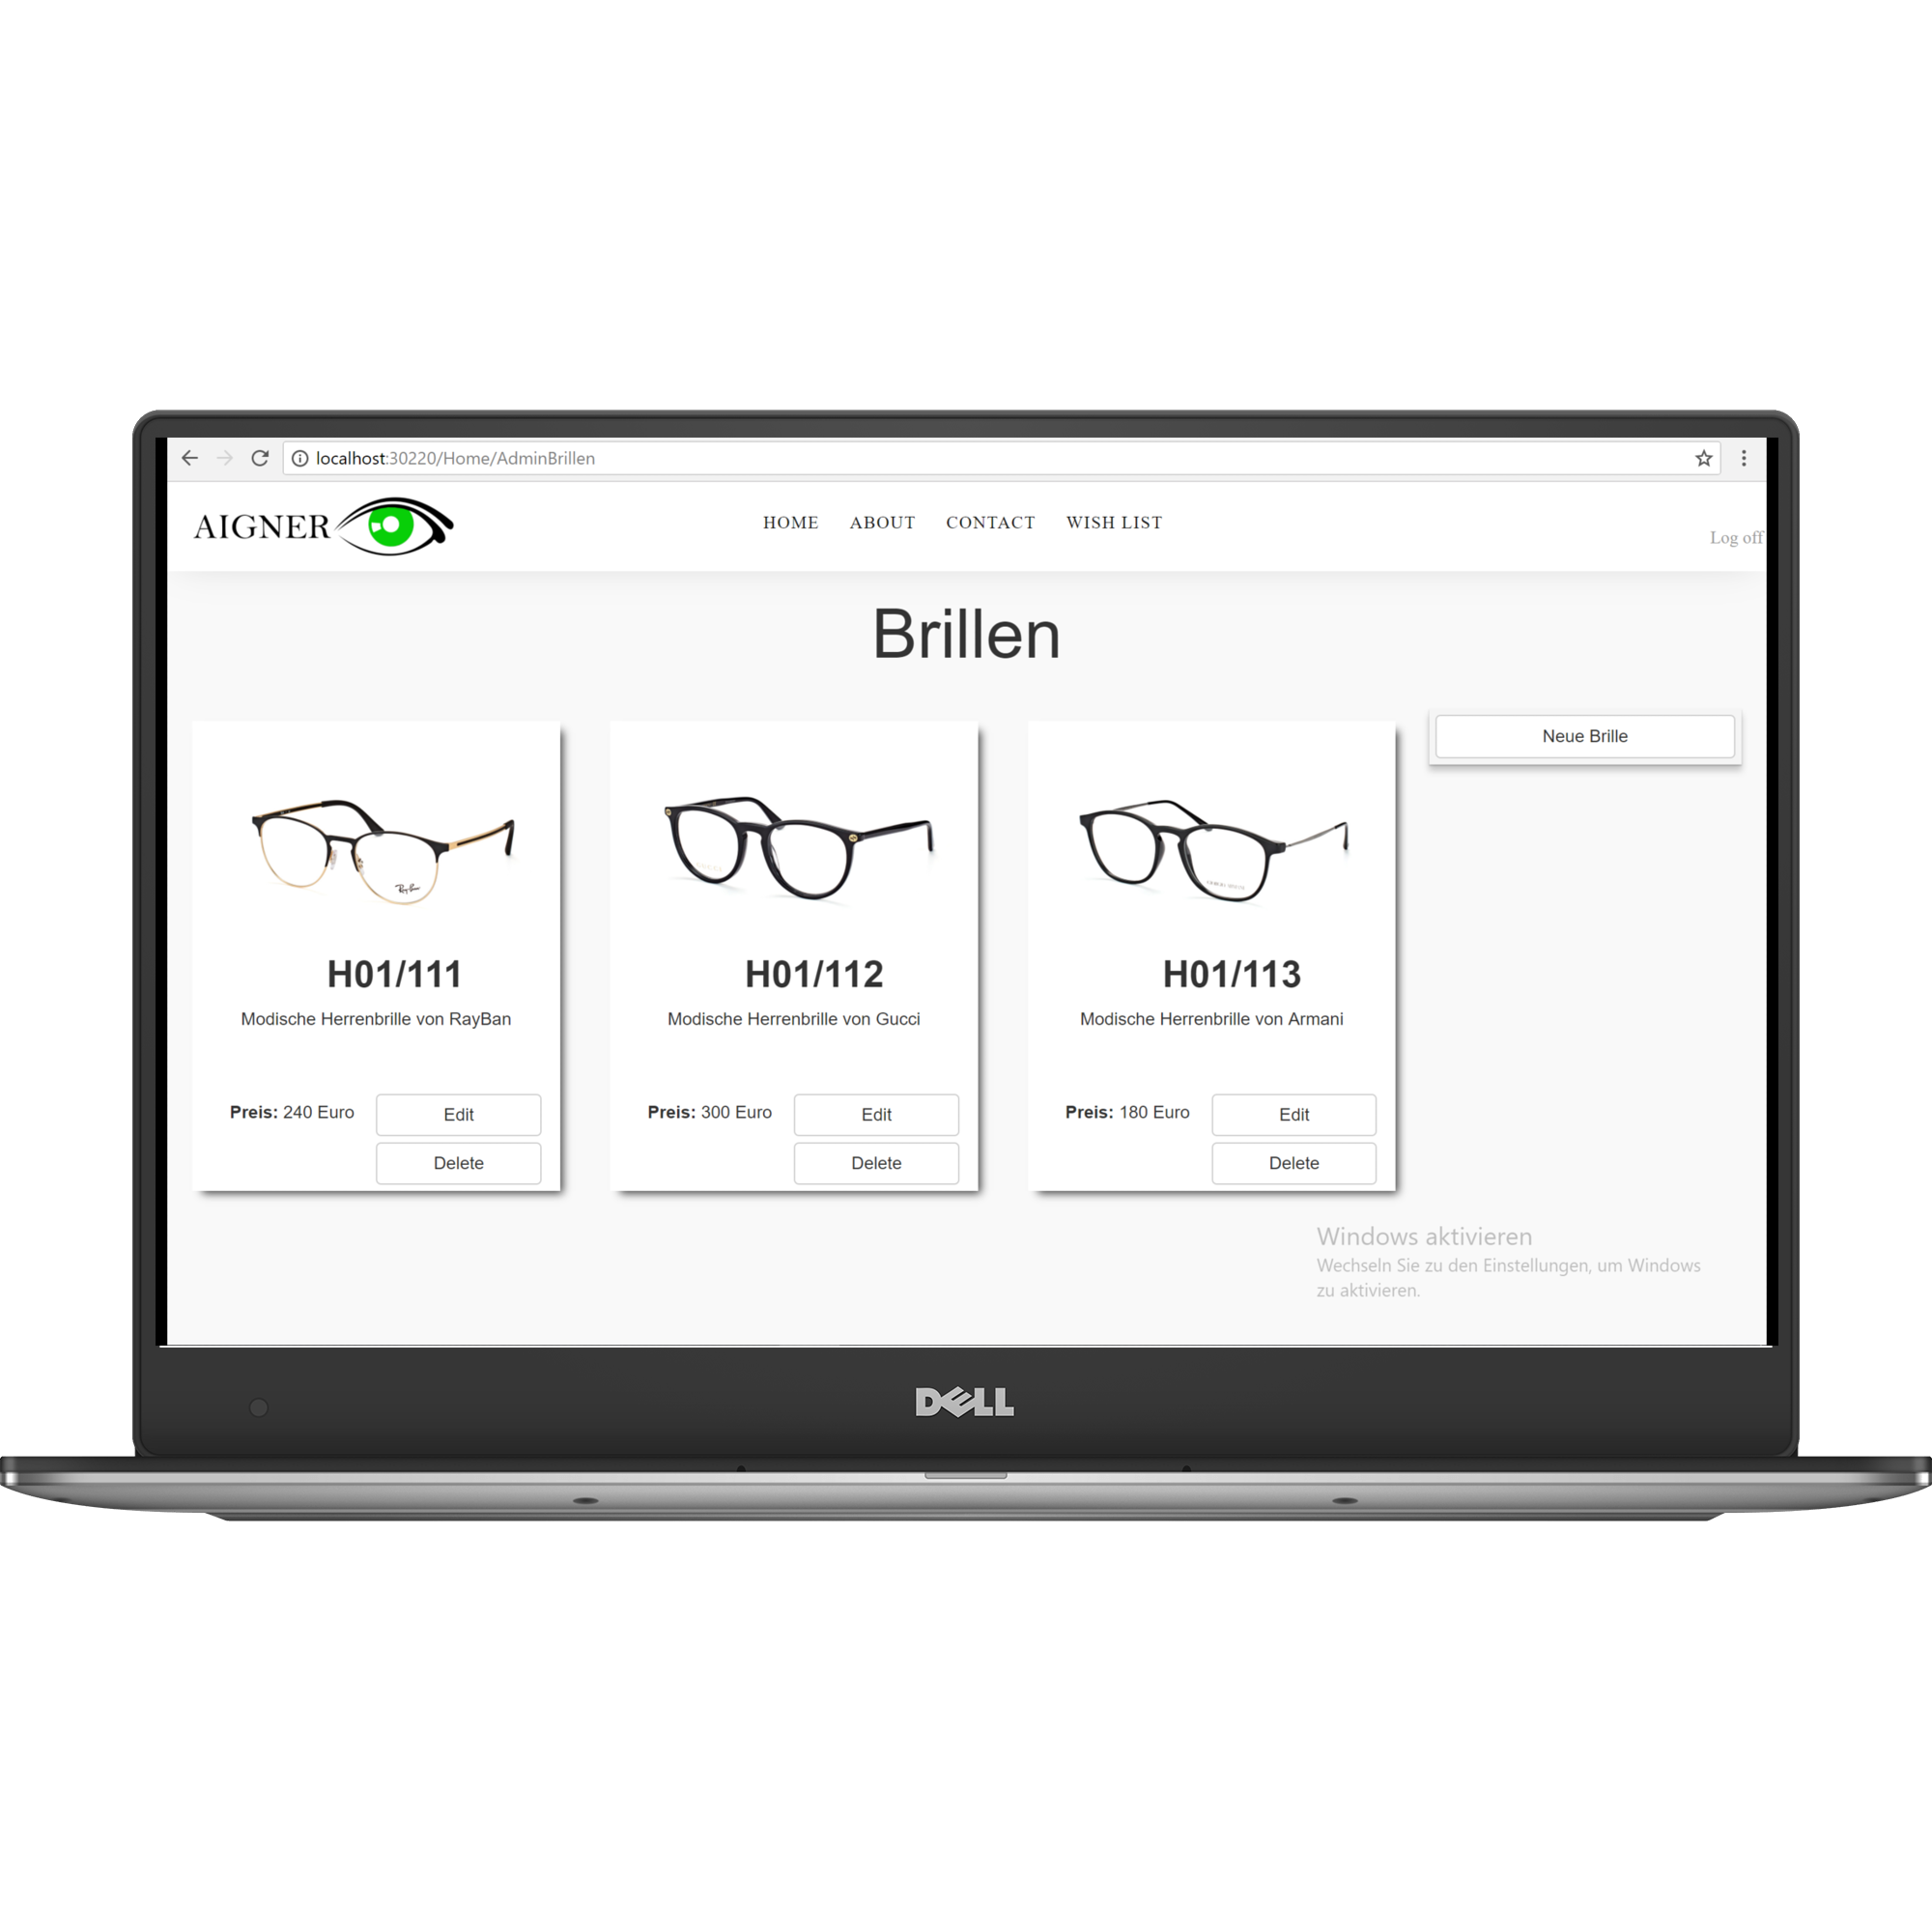
\includegraphics[scale=.2]{images/AdminBrillen.png}
\end{center}
	\caption{Model-View-Controller Konzept}
	\label{fig:sample}
\end{figure}

\subsubsection{Brille hinzufügen}
Auf dieser Seite kann der Administrator neue Brillenmodelle einfügen dazu muss er den Titel und den Preis eingeben und ein Foto der Brille einfügen, dann kann er auf "Brille hinzufügen" drücken. Dies führt dazu, dass die Brille in der Datenbank eingefügt wird und dass er auf die Seite "Brillen" zurückkehrt wo die aktualisierte Liste der Brillen zu sehen ist.

\subsubsection{Brille bearbeiten}
Auf dieser Seite kann der Administrator den eingegebenen Titel, den Preis oder auch das Bild einer bereits vorhandenen Brille ändern. Nachdem die Änderungen vorgenommen wurden und er diese mit dem "Brille bearbeiten" Button bestätigt wird der Administrator automatisch auf die Seite "Brillen" zurückkehren wo die aktualisierte Liste aller Brillen zu sehen ist.

\section{Allgemeine Informationen}
Um allgemeinen Informationen über das Unternehmen zu erhalten, gibt es einen Menüpunkt "About", hier werden alle Informationen wie die Öffnungszeiten, Fax-, Mobil- und die Telefonnummer angezeigt, außerdem wird der Standort des Unternehmens auf einer eingebunden Google Maps Karte dargestellt.

\begin{figure}[H]
\begin{center}
	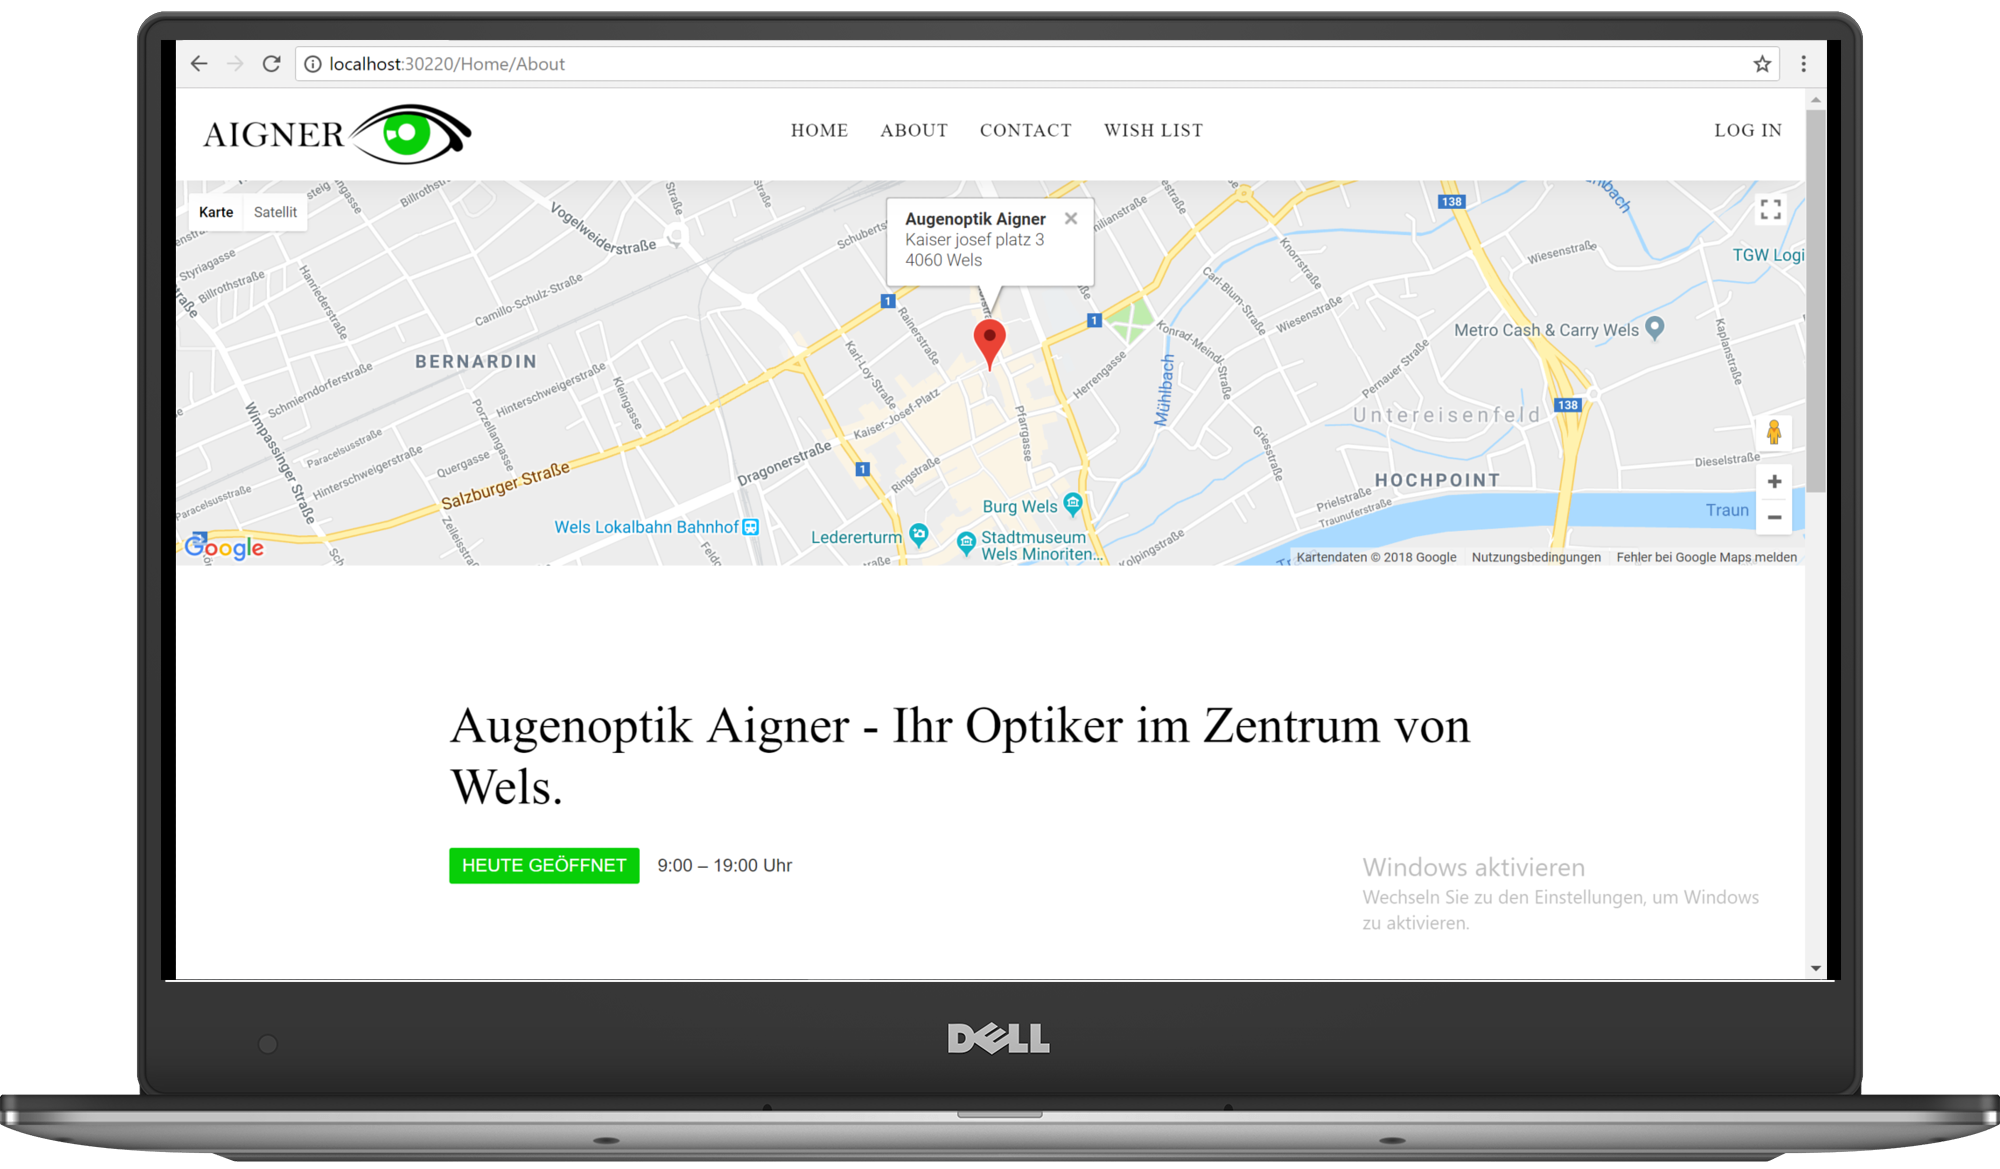
\includegraphics[scale=.2]{images/About.png}
\end{center}
	\caption{Model-View-Controller Konzept}
	\label{fig:sample}
\end{figure}

\section{Kontakt}
Bei Fragen über die Website, das Unternehmen, die Brillenmodelle und allem anderen kann der Verkäufer mittels eines Formulars kontaktiert werden. Um zum Kontaktformular zu gelangen gibt es in der Navigation bar den Punkt "Kontakt". Dort gibt man seinen Namen, die eigene E-mail Adresse und die Nachricht ein und das Formular kann dann gesendet werden. Die eingegeben Nachricht wird dann über einen SMTP Server an die E-Mail Adresse des Verkäufers gesendet. Die Mail beinhaltet die Nachricht sowie den eingegebenen Namen und auch die E-Mail Adresse somit kann der Verkäufer auf die erhaltene Nachricht antworten.

\begin{figure}[H]
\begin{center}
	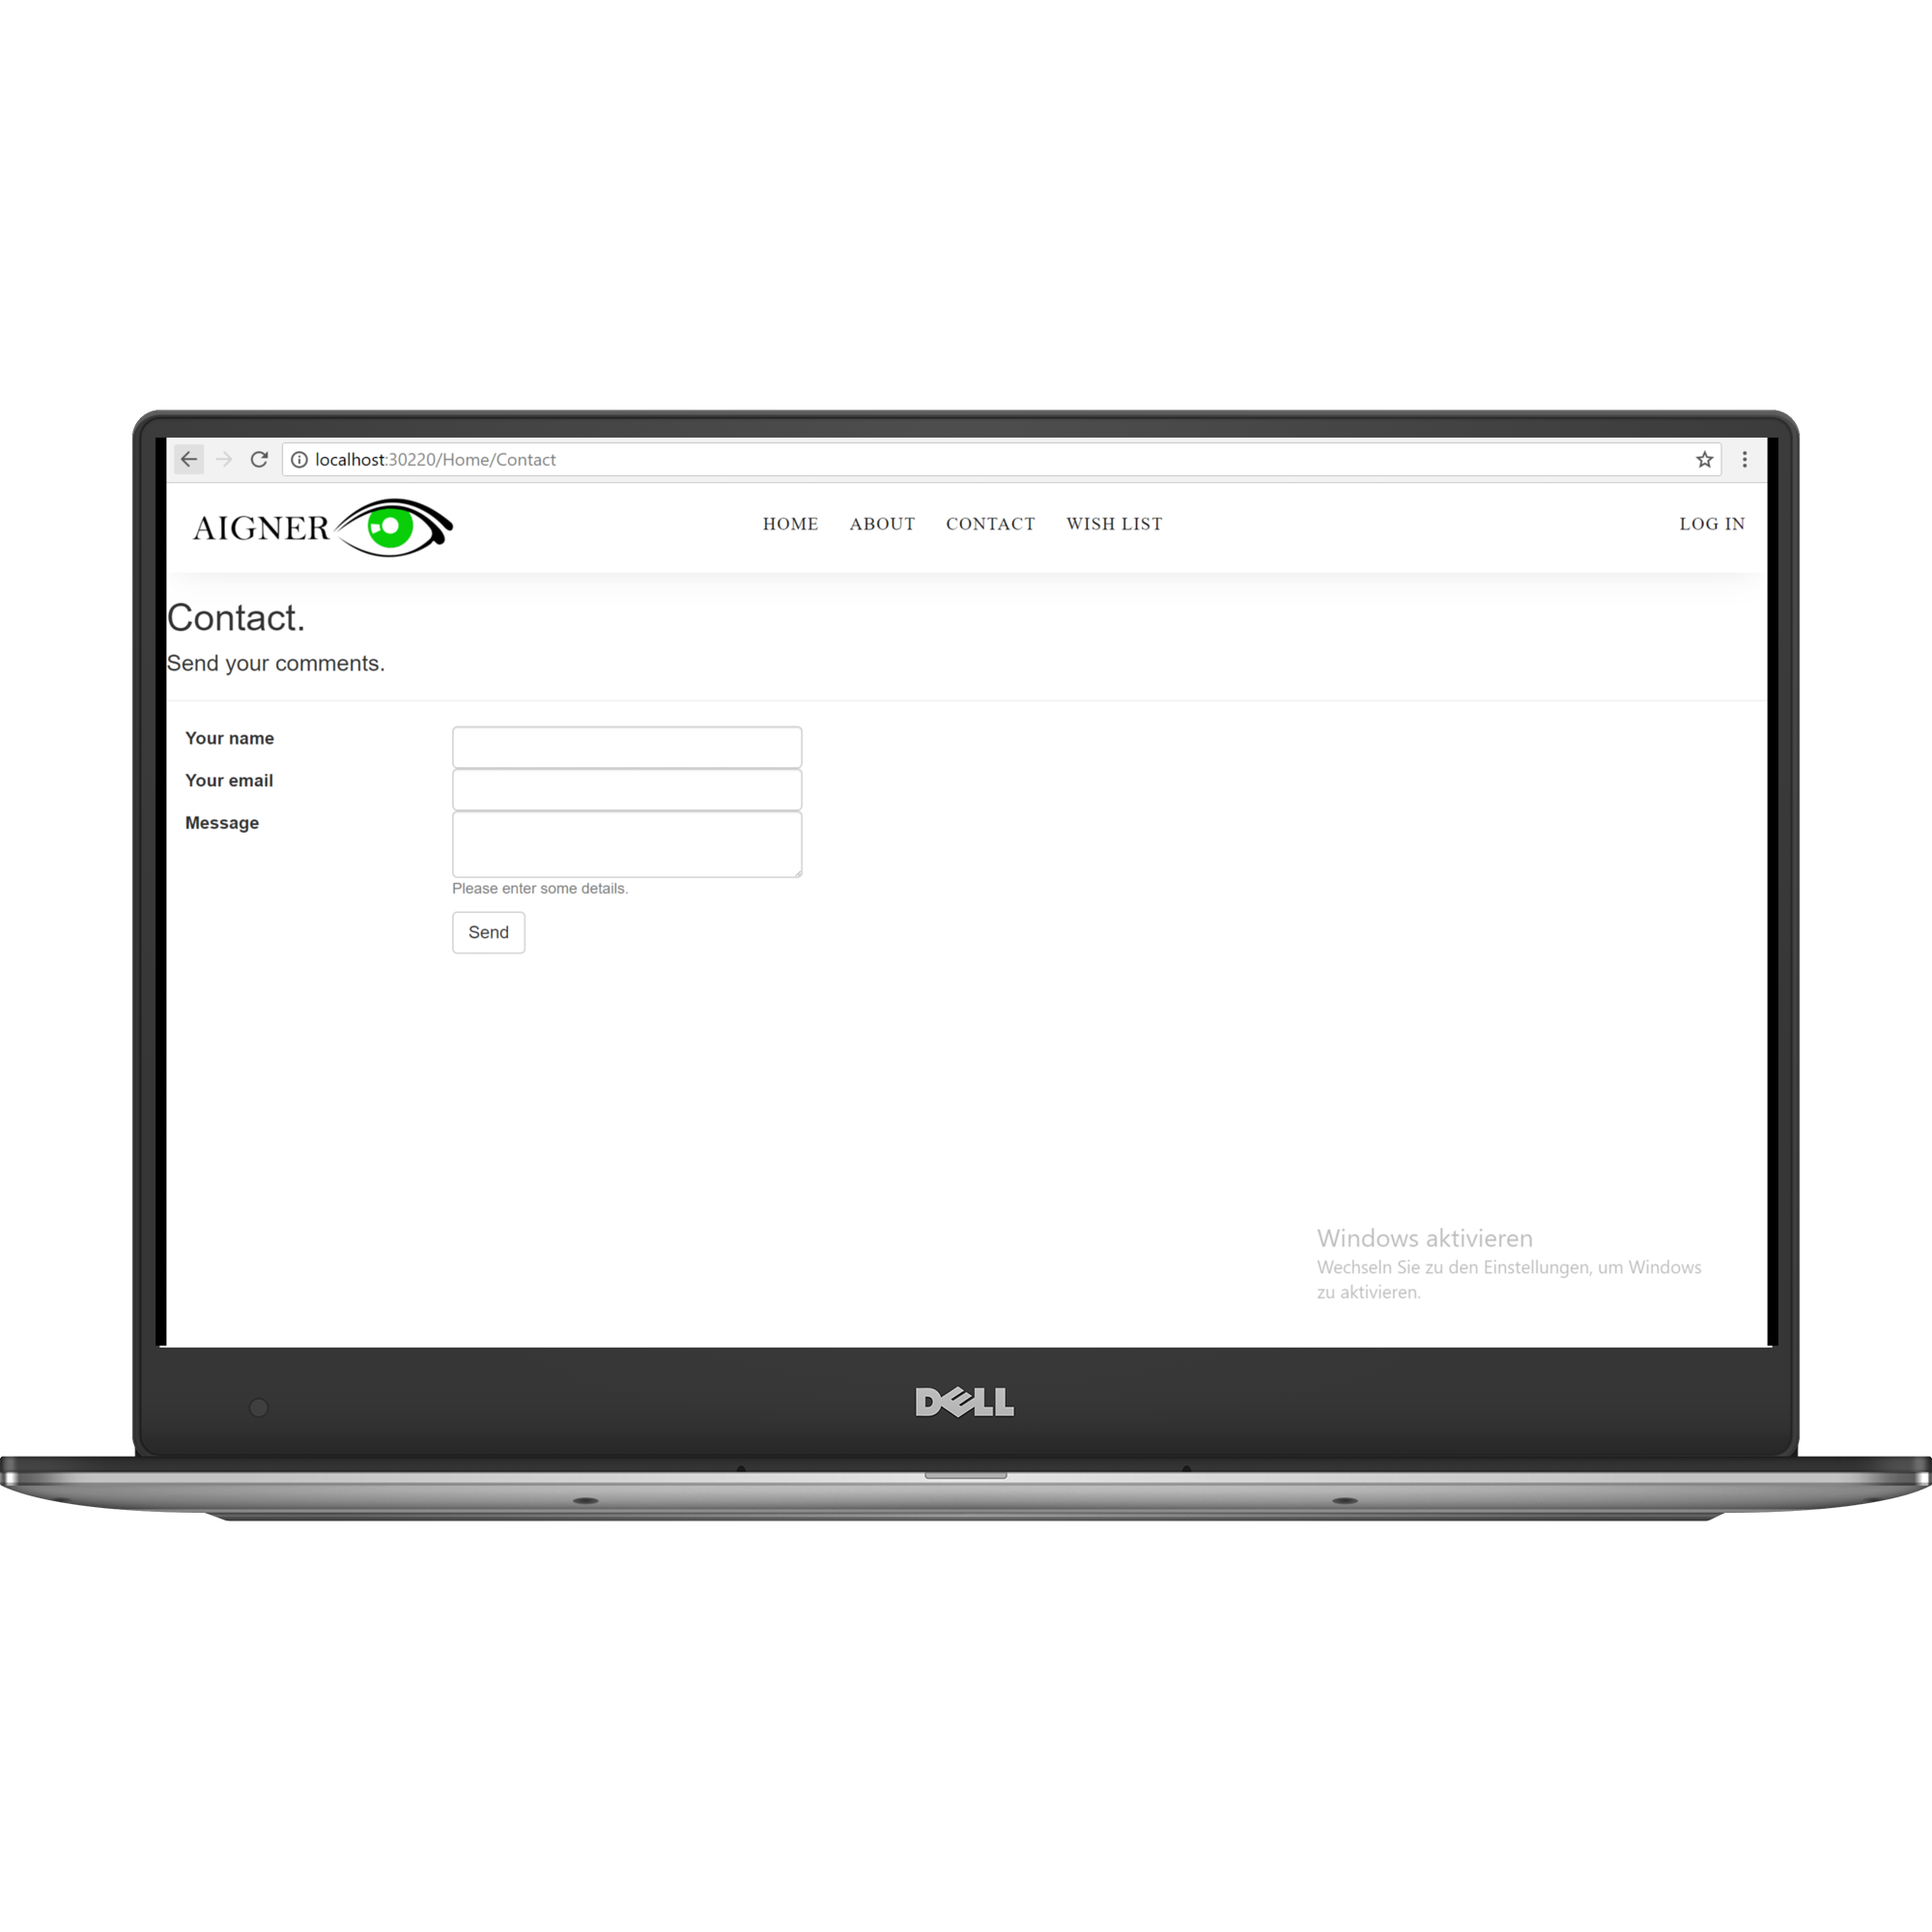
\includegraphics[scale=.2]{images/Contact.png}
\end{center}
	\caption{Model-View-Controller Konzept}
	\label{fig:sample}
\end{figure}



